% Title     :: SamzaSQL: Scalable Fast Data Management with Streaming SQL
% Author    :: Milinda Pathirage
% Email     :: mpathira@indiana.edu
% Website   :: http://milinda.pathirage.org
% Template  :: sthlm beamer theme by Benjamin Weiss (hendryolson@gmail.com, http://v42.com), 
%              which is HEAVILY based on the HSRM beamer theme created by Benjamin Weiss
%			   (benjamin.weiss@student.hs-rm.de), which can be found on GitHub
%			   <https://github.com/hsrmbeamertheme/hsrmbeamertheme>.



%-=-=-=-=-=-=-=-=-=-=-=-=-=-=-=-=-=-=-=-=-=-=-=-=
%
%        LOADING DOCUMENT
%
%-=-=-=-=-=-=-=-=-=-=-=-=-=-=-=-=-=-=-=-=-=-=-=-=

\documentclass[newPxFont]{beamer}
\usetheme{sthlm}
%\usecolortheme{sthlmv42}

%-=-=-=-=-=-=-=-=-=-=-=-=-=-=-=-=-=-=-=-=-=-=-=-=
%        LOADING PACKAGES
%-=-=-=-=-=-=-=-=-=-=-=-=-=-=-=-=-=-=-=-=-=-=-=-=
\usepackage[utf8]{inputenc}
\usepackage{hyperref}
\usepackage{minted}
\usepackage{xcolor}

\usepackage{chronology}

\renewcommand{\event}[3][e]{%
  \pgfmathsetlength\xstop{(#2-\theyearstart)*\unit}%
  \ifx #1e%
    \draw[fill=black,draw=none,opacity=0.5]%
      (\xstop, 0) circle (.2\unit)%
      node[opacity=1,rotate=45,right=.2\unit] {#3};%
  \else%
    \pgfmathsetlength\xstart{(#1-\theyearstart)*\unit}%
    \draw[fill=black,draw=none,opacity=0.5,rounded corners=.1\unit]%
      (\xstart,-.1\unit) rectangle%
      node[opacity=1,rotate=45,right=.2\unit] {#3} (\xstop,.1\unit);%
  \fi}%

%-=-=-=-=-=-=-=-=-=-=-=-=-=-=-=-=-=-=-=-=-=-=-=-=
%        BEAMER OPTIONS
%-=-=-=-=-=-=-=-=-=-=-=-=-=-=-=-=-=-=-=-=-=-=-=-=

%\setbeameroption{show notes}

%-=-=-=-=-=-=-=-=-=-=-=-=-=-=-=-=-=-=-=-=-=-=-=-=
%
%	PRESENTATION INFORMATION
%
%-=-=-=-=-=-=-=-=-=-=-=-=-=-=-=-=-=-=-=-=-=-=-=-=

\title{SamzaSQL}
\subtitle{Scalable Fast Data Management with \textit{Streaming SQL}}
%\date{\small{\jobname}}
%\date{\today}
\author{\textbf{Milinda Pathirage} (IU), Julian Hyde (Hortonworks), Yi Pan (LinkedIn), Beth Plale (IU)}
\institute{School of Informatics and Computing, Indiana University}

\hypersetup{
pdfauthor = {Milinda Pathirage: mpathira@indiana.edu},
pdfsubject = {},
pdfkeywords = {},
pdfmoddate= {D:\pdfdate},
pdfcreator = {}
}

\begin{document}
\setbeamertemplate{caption}{\raggedright\insertcaption\par}

%-=-=-=-=-=-=-=-=-=-=-=-=-=-=-=-=-=-=-=-=-=-=-=-=
%
%	TITLE PAGE
%
%-=-=-=-=-=-=-=-=-=-=-=-=-=-=-=-=-=-=-=-=-=-=-=-=

\maketitle

%\begin{frame}[plain]
%	\titlepage
%\end{frame}

%-=-=-=-=-=-=-=-=-=-=-=-=-=-=-=-=-=-=-=-=-=-=-=-=
%
%	TABLE OF CONTENTS: OVERVIEW
%
%-=-=-=-=-=-=-=-=-=-=-=-=-=-=-=-=-=-=-=-=-=-=-=-=

\section*{Introduction}

%-=-=-=-=-=-=-=-=-=-=-=-=-=-=-=-=-=-=-=-=-=-=-=-=
%	FRAME:
%-=-=-=-=-=-=-=-=-=-=-=-=-=-=-=-=-=-=-=-=-=-=-=-=

\begin{frame}[c]{Fast Data}

Data has to be process as it arrives, so that we can react to changing conditions fast. 

\vspace{1em}

\begin{exampleblock}{Big data isn't just big; it's also fast.}
Big data is often created by data that is generated at incredible speeds, such as click-stream data, financial ticker data, log aggregation, or sensor data. 
\end{exampleblock}
\vspace{-1.5em}
\begin{flushright}
\tiny\textit{John Hugg, \textbf{"Fast data: The next step after big data"}}
\end{flushright}

\end{frame}

%-=-=-=-=-=-=-=-=-=-=-=-=-=-=-=-=-=-=-=-=-=-=-=-=
%	FRAME:
%-=-=-=-=-=-=-=-=-=-=-=-=-=-=-=-=-=-=-=-=-=-=-=-=

\begin{frame}[c]{Lambda Architecture (LA)}
Technology agnostic data processing architecture that attempts to balance latency, accuracy, throughput and fault-tolerance by providing a unified serving layer on top of batch and stream processing sub-systems.   \\

\vspace{1em}

\begin{figure}
		\centering
		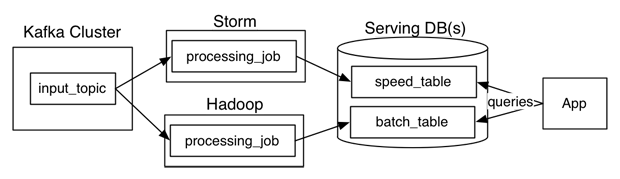
\includegraphics[width=0.75\linewidth]{lambda.png}
		\label{fig-lambda}
		\caption{\tiny\textit{From: \url{https://www.oreilly.com/ideas/questioning-the-lambda-architecture}}}
	\end{figure}

\end{frame}

%-=-=-=-=-=-=-=-=-=-=-=-=-=-=-=-=-=-=-=-=-=-=-=-=
%	FRAME:
%-=-=-=-=-=-=-=-=-=-=-=-=-=-=-=-=-=-=-=-=-=-=-=-=

\begin{frame}[c]{Kappa Architecture (KA)}
Simplification of \textit{Lambda Architecture} that uses append-only immutable log as the canonical data store and batch processing is replaced by stream replay. \\

\vspace{1em}

\begin{figure}
		\centering
		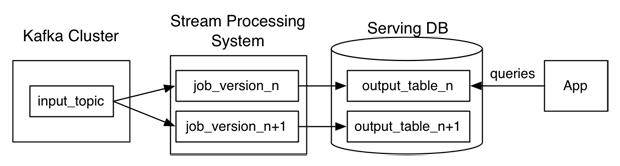
\includegraphics[width=0.75\linewidth]{kappa.png}
		\label{fig-lambda}
		\caption{\tiny\textit{From: \url{https://www.oreilly.com/ideas/questioning-the-lambda-architecture}}}
	\end{figure}

\end{frame}

%-=-=-=-=-=-=-=-=-=-=-=-=-=-=-=-=-=-=-=-=-=-=-=-=
%	FRAME:
%-=-=-=-=-=-=-=-=-=-=-=-=-=-=-=-=-=-=-=-=-=-=-=-=

%\begin{frame}[c]{sthlm Built on HSRM \& mTheme}
%\vspace{-1cm}
%\begin{center}\begin{chronology}[2]{2012}{2018}{0.85\textwidth}
%\event[\decimaldate{1}{1}{2013}]{\decimaldate{22}{9}{2013}}{hsrm theme}
%\event[\decimaldate{22}{9}{2013}]{\decimaldate{22}{8}{2014}}{sthlm based on hsrm}
%\event[\decimaldate{22}{8}{2014}]{\decimaldate{27}{4}{2015}}{branding sthlm for Stockholms stad}
%\event[\decimaldate{27}{4}{2015}]{\decimaldate{30}{8}{2015}}{\cRed{sthlm based on hsrm \& mTheme}}
%\end{chronology}
%\end{center}

%sthlm Theme is heavily based on the work of Benjamin Weiss \alert{HSRM} and Matthias Vogelgesang \alert{mTheme}.

%\end{frame}

%\section*{Overview}
%\begin{frame}{Overview}
% For longer presentations use hideallsubsections option
%\tableofcontents[hideallsubsections]
%\end{frame}


%-=-=-=-=-=-=-=-=-=-=-=-=-=-=-=-=-=-=-=-=-=-=-=-=
%
%	SECTION: Motivation
%
%-=-=-=-=-=-=-=-=-=-=-=-=-=-=-=-=-=-=-=-=-=-=-=-=

\section*{Motivation}

%-=-=-=-=-=-=-=-=-=-=-=-=-=-=-=-=-=-=-=-=-=-=-=-=
%	FRAME:
%-=-=-=-=-=-=-=-=-=-=-=-=-=-=-=-=-=-=-=-=-=-=-=-=

\begin{frame}{SQL for Big Data}

There are sevaral well known SQL-on-Hadoop solutions and most organisations that use Hadoop use one or more SQL-on-Hadoop solutions.

\begin{itemize}
	\item Apache Hive
	\item Presto
	\item Apache Drill
	\item Apache Impala
	\item Apache Kylin
	\item Apache Tajo
	\item Apache Pheonix
\end{itemize}

\end{frame}

%-=-=-=-=-=-=-=-=-=-=-=-=-=-=-=-=-=-=-=-=-=-=-=-=
%	FRAME: 
%-=-=-=-=-=-=-=-=-=-=-=-=-=-=-=-=-=-=-=-=-=-=-=-=

\begin{frame}{Programming APIs for LA and KA}

\href{https://github.com/twitter/summingbird}{\textbf{Summingbird}} is a well known abstraction for writing \textit{LA} style applications while \textit{KA} style applications were mainly written in \textbf{stateful stream processing APIs} provided by frameworks like \href{http://samza.apache.org}{Apache Samza}.

\begin{block}{Limitations}
\begin{itemize}
	\item Need to maintain two complex distributed systems
	\item Users need to understand various programming abstractions 
	\item Long turnaround times
\end{itemize}
\end{block}

\end{frame}

%-=-=-=-=-=-=-=-=-=-=-=-=-=-=-=-=-=-=-=-=-=-=-=-=
%	FRAME: 
%-=-=-=-=-=-=-=-=-=-=-=-=-=-=-=-=-=-=-=-=-=-=-=-=

\begin{frame}[fragile]{Summingbird}
\begin{exampleblock}{Word Count}
\begin{minted}[
framesep=2mm,
baselinestretch=1.2,
fontsize=\footnotesize,
]{scala}
def wordCount[P <: Platform[P]]
    (source: Producer[P, String], store: P#Store[String, Long]) =
      source.flatMap { sentence =>
        toWords(sentence).map(_ -> 1L)
      }.sumByKey(store)
\end{minted}
\end{exampleblock}

\end{frame}

\begin{frame}{Motivating Research Question}
\Large\textbf{Can the same low barrier and the clear semantics of SQL be extended to queries that execute simultaneously over data streams (in movement) and tables (at rest)?} \\

\Large\textbf{Can this be done with minimal and well-founded extensions to SQL?}
\end{frame}
%-=-=-=-=-=-=-=-=-=-=-=-=-=-=-=-=-=-=-=-=-=-=-=-=
%
%	SECTION: UPDATESS
%
%-=-=-=-=-=-=-=-=-=-=-=-=-=-=-=-=-=-=-=-=-=-=-=-=

\section{Updates}

%-=-=-=-=-=-=-=-=-=-=-=-=-=-=-=-=-=-=-=-=-=-=-=-=
%	FRAME:
%-=-=-=-=-=-=-=-=-=-=-=-=-=-=-=-=-=-=-=-=-=-=-=-=

\begin{frame}[c]{Version 0.6}
\alert{NeW} in version 0.6

\begin{itemize}
	\item \texttt{beamerthemesthlm.sty}
	\begin{itemize}
		\item Removed log from header
		\item Removed vertically aligned columns support
		\item Removed listings package support
		\item Added PxFont option to use the fonts:
		\begin{itemize}
			\item newpxtext
			\item newpxmath
		\end{itemize}
	\end{itemize}
\end{itemize}
\end{frame}


%-=-=-=-=-=-=-=-=-=-=-=-=-=-=-=-=-=-=-=-=-=-=-=-=
%
%	SECTION: STRUCTURE
%
%-=-=-=-=-=-=-=-=-=-=-=-=-=-=-=-=-=-=-=-=-=-=-=-=
\section{Colors}

%-=-=-=-=-=-=-=-=-=-=-=-=-=-=-=-=-=-=-=-=-=-=-=-=
%	FRAME:
%-=-=-=-=-=-=-=-=-=-=-=-=-=-=-=-=-=-=-=-=-=-=-=-=

\begin{frame}[containsverbatim,c]{Color Style File}

The sthlm theme style file \texttt{beamerthemesthlm.sty} references the \texttt{beamercolorthemesthlm.sty} file for the theme colors.

\vspace{1em}

\begin{block}{Note:}
The original sthlm color theme can now be used in place of Stockholm Stads color palette by including \newline \lstinline!\usecolortheme{sthlmv42}! in the preamble.
\end{block}

\end{frame}

%-=-=-=-=-=-=-=-=-=-=-=-=-=-=-=-=-=-=-=-=-=-=-=-=
%	FRAME:
%-=-=-=-=-=-=-=-=-=-=-=-=-=-=-=-=-=-=-=-=-=-=-=-=

\begin{frame}[c]{Primary Presentation Colors}

\begin{columns}[c]

%	Color Box: Dark Grey
\begin{column}{0.23\textwidth}
\setbeamercolor{boxsthlmDarkGrey}{bg=\cnDarkGrey,fg=white}
\begin{beamercolorbox}[wd=\linewidth,ht=10ex,dp=3ex]{boxsthlmDarkGrey}
\centering
	\texttt{DarkGrey}\\
	\vspace{1em}
	\tiny{RGB:  51, 51 , 51} \\
	\tiny{hex: \#333333}
\end{beamercolorbox}

\vspace{3em}

%	Color Box: Grey
\setbeamercolor{boxsthlmGrey}{bg=\cnGrey,fg=sthlmDarkGrey}
\begin{beamercolorbox}[wd=\linewidth,ht=10ex,dp=3ex]{boxsthlmGrey}
\centering
	\texttt{Grey}\\
	\vspace{1em}
	\tiny{RGB:  245,243,238} \\
	\tiny{hex: \#f5f3ee}
\end{beamercolorbox}

\end{column}

\begin{column}{0.23\textwidth}

%	Color Box: Blue
\setbeamercolor{boxsthlmBlue}{bg=\cnBlue,fg=white}
\begin{beamercolorbox}[wd=\linewidth,ht=10ex,dp=3ex]{boxsthlmBlue}
\centering
	\texttt{Blue}\\
	\vspace{1em}
	\tiny{RGB:  0,110,191} \\
	\tiny{hex: \#006ebf}
\end{beamercolorbox}

\vspace{3em}

%	Color Box: Light Blue
\setbeamercolor{boxsthlmLightBlue}{bg=\cnLightBlue,fg=sthlmDarkGrey}
\begin{beamercolorbox}[wd=\linewidth,ht=10ex,dp=3ex]{boxsthlmLightBlue}
\centering
	\texttt{Light Blue}\\
	\vspace{1em}
	\tiny{RGB:  214,237,252} \\
	\tiny{hex: \#d6edfc}
\end{beamercolorbox}
\end{column}

\begin{column}{0.23\textwidth}

%	Color Box: Red
\setbeamercolor{boxsthlmRed}{bg=\cnRed,fg=white}
\begin{beamercolorbox}[wd=\linewidth,ht=10ex,dp=3ex]{boxsthlmRed}
\centering
	\texttt{Red}\\
	\vspace{1em}
	\tiny{RGB:  196,0,100} \\
	\tiny{hex: \#c40064}
\end{beamercolorbox}

\vspace{3em}

%	Color Box: Light Red
\setbeamercolor{boxsthlmLightRed}{bg=\cnLightRed,fg=sthlmDarkGrey}
\begin{beamercolorbox}[wd=\linewidth,ht=10ex,dp=3ex]{boxsthlmLightRed}
\centering
	\texttt{Light Red}\\
	\vspace{1em}
	\tiny{RGB:  254,222,237} \\
	\tiny{hex: \#fedeed}
\end{beamercolorbox}
\end{column}


\begin{column}{0.23\textwidth}
%	Color Box: Green
\setbeamercolor{boxsthlmGreen}{bg=\cnGreen,fg=white}
\begin{beamercolorbox}[wd=\linewidth,ht=10ex,dp=3ex]{boxsthlmGreen}
\centering
	\texttt{Green}\\
	\vspace{1em}
	\tiny{RGB:  0,134,127} \\
	\tiny{hex: \#00867f}
\end{beamercolorbox}

\vspace{3em}

%	Color Box: Light Green
\setbeamercolor{boxsthlmLightGreen}{bg=\cnLightGreen,fg=sthlmDarkGrey}
\begin{beamercolorbox}[wd=\linewidth,ht=10ex,dp=3ex]{boxsthlmLightGreen}
\centering
	\texttt{Light Green}\\
	\vspace{1em}
	\tiny{RGB:  0,134,127} \\
	\tiny{hex: \#d5f7f4}
\end{beamercolorbox}
\end{column}
\end{columns}


\end{frame}

%-=-=-=-=-=-=-=-=-=-=-=-=-=-=-=-=-=-=-=-=-=-=-=-=
%	Secondary Colors:
%-=-=-=-=-=-=-=-=-=-=-=-=-=-=-=-=-=-=-=-=-=-=-=-=

\begin{frame}[c]{Secondary Presentation Colors}

\begin{columns}[c]

%	Color Box: Orange
\begin{column}{0.23\textwidth}
\setbeamercolor{boxsthlmOrange}{bg=\cnOrange,fg=white}
\begin{beamercolorbox}[wd=\linewidth,ht=10ex,dp=3ex]{boxsthlmOrange}
\centering
	\texttt{Orange}\\
	\vspace{1em}
	\tiny{RGB:  221,74,44} \\
	\tiny{hex: \#dd4a2c}
\end{beamercolorbox}

\vspace{3em}

%	Color Box: Light Orange
\setbeamercolor{boxsthlmLightOrange}{bg=\cnLightOrange,fg=sthlmDarkGrey}
\begin{beamercolorbox}[wd=\linewidth,ht=10ex,dp=3ex]{boxsthlmLightOrange}
\centering
	\texttt{Light Orange}\\
	\vspace{1em}
	\tiny{RGB:  255,215,210} \\
	\tiny{hex: \#ffd7d2}
\end{beamercolorbox}

\end{column}

%	Color Box: Purple
\begin{column}{0.23\textwidth}
\setbeamercolor{boxsthlmPurple}{bg=\cnPurple,fg=white}
\begin{beamercolorbox}[wd=\linewidth,ht=10ex,dp=3ex]{boxsthlmPurple}
\centering
	\texttt{Purple}\\
	\vspace{1em}
	\tiny{RGB:  93,35,125} \\
	\tiny{hex: \#5d237d}
\end{beamercolorbox}

\vspace{3em}

%	Color Box: Light Purple
\setbeamercolor{boxsthlmLightPurple}{bg=\cnLightPurple,fg=sthlmDarkGrey}
\begin{beamercolorbox}[wd=\linewidth,ht=10ex,dp=3ex]{boxsthlmLightPurple}
\centering
	\texttt{Light Purple}\\
	\vspace{1em}
	\tiny{RGB:  241,230,252} \\
	\tiny{hex: \#f1e6fc}
\end{beamercolorbox}
\end{column}

\begin{column}{0.23\textwidth}

%	Color Box: Yellow
\setbeamercolor{boxsthlmYellow}{bg=\cnYellow,fg=white}
\begin{beamercolorbox}[wd=\linewidth,ht=10ex,dp=3ex]{boxsthlmYellow}
\centering
	\texttt{Yellow}\\
	\vspace{1em}
	\tiny{RGB:  252,191,10} \\
	\tiny{hex: \#fcbf0a}
\end{beamercolorbox}

\vspace{3em}

%	Color Box: BLANK
\setbeamercolor{boxsthlmBlank}{bg=\cnGrey, fg=\cnGrey}
\begin{beamercolorbox}[wd=\linewidth,ht=10ex,dp=3ex]{boxsthlmBlank}
\centering
	\texttt{Yellow}\\
	\vspace{1em}
	\tiny{RGB} \\
	\tiny{hex}
\end{beamercolorbox}
\end{column}


\begin{column}{0.23\textwidth}
%	Color Box: issr Blue
\setbeamercolor{boxsthlmissrBlue}{bg=issrBlue,fg=white}
\begin{beamercolorbox}[wd=\linewidth,ht=10ex,dp=3ex]{boxsthlmissrBlue}
\centering
	\texttt{ISSR Blue}\\
	\vspace{1em}
	\tiny{RGB:  0,111,174} \\
	\tiny{hex: \#0066cc}
\end{beamercolorbox}

\vspace{3em}

%	Color Box: issr Grey
\setbeamercolor{boxsthlmissrGrey}{bg=issrGrey,fg=sthlmDarkGrey}
\begin{beamercolorbox}[wd=\linewidth,ht=10ex,dp=3ex]{boxsthlmissrGrey}
\centering
	\texttt{ISSR Grey}\\
	\vspace{1em}
	\tiny{RGB:  167,169,172} \\
	\tiny{hex: \#999999}
\end{beamercolorbox}
\end{column}
\end{columns}

\end{frame}

%-=-=-=-=-=-=-=-=-=-=-=-=-=-=-=-=-=-=-=-=-=-=-=-=
%	FRAME: Theme Package Requirements
%-=-=-=-=-=-=-=-=-=-=-=-=-=-=-=-=-=-=-=-=-=-=-=-=

\begin{frame}[containsverbatim]{Theme Package Requirements}

This theme requires that the following packages are installed:

\begin{columns}[t]
\begin{column}{0.5\textwidth}
\begin{itemize}
\item \lstinline!{beamer}!
\item \lstinline!{calc}!
\item \lstinline!{eso-pic}!
\item \lstinline![utf8]{inputenc}!
\end{itemize}
\end{column}

\begin{column}{0.5\textwidth}
\begin{itemize}
\item \lstinline!{listings}!
\item \lstinline!{pgf}!
\item \lstinline!{xcolor}!
\end{itemize}
\end{column}
\end{columns}

\end{frame}


%-=-=-=-=-=-=-=-=-=-=-=-=-=-=-=-=-=-=-=-=-=-=-=-=
%	FRAME: Theme Package Requirements
%-=-=-=-=-=-=-=-=-=-=-=-=-=-=-=-=-=-=-=-=-=-=-=-=
\begingroup
\setbeamercolor{background canvas}{bg=\cnLightRed}
\begin{frame}[containsverbatim]{Frame Colored Backgrounds}

You can change the color of a frame background by placing the frame within a group:

\begin{sthlmLatex}

\begingroup
\setbeamercolor{background canvas}{bg=sthlmLightRed}
\begin{frame}
	% Your frame content goes here
\end{frame}
\endgroup
\end{sthlmLatex}

\end{frame}
\endgroup

%-=-=-=-=-=-=-=-=-=-=-=-=-=-=-=-=-=-=-=-=-=-=-=-=
%	FRAME: Theme Package Requirements
%-=-=-=-=-=-=-=-=-=-=-=-=-=-=-=-=-=-=-=-=-=-=-=-=
\begingroup
\setbeamercolor{background canvas}{bg=\cnBlue}
\begin{frame}[plain,containsverbatim]

Or maybe you want a blank blue frame to work with

\begin{sthlmLatex}

\begingroup
\setbeamercolor{background canvas}{bg=sthlmBlue}
\begin[plain]{frame}
	% Your frame content goes here
\end{frame}
\endgroup
\end{sthlmLatex}

\end{frame}
\endgroup

%-=-=-=-=-=-=-=-=-=-=-=-=-=-=-=-=-=-=-=-=-=-=-=-=
%	FRAME: Theme Fonts
%-=-=-=-=-=-=-=-=-=-=-=-=-=-=-=-=-=-=-=-=-=-=-=-=

\begin{frame}[containsverbatim]{Theme Fonts}

To use the newpx fonts option you need the following packages:

\begin{itemize}
	\item \verb|{newpxtext}|
	\item \verb|{newpxmath}|
	\item \verb|[T1]{fontenc}|
\end{itemize}

To enable the \verb|newpxtext| and \verb|newpxmath| fonts include the \alert{PxFont} class option.\\

\begin{itemize}
	\item \verb|\documentclass[compress,PxFont]{beamer}|
\end{itemize}

\end{frame}

%-=-=-=-=-=-=-=-=-=-=-=-=-=-=-=-=-=-=-=-=-=-=-=-=
%	FRAME: Theme Options
%-=-=-=-=-=-=-=-=-=-=-=-=-=-=-=-=-=-=-=-=-=-=-=-=

\begin{frame}{Theme Options}
\begin{table}[]
	\begin{tabularx}{\linewidth}{l>{\raggedright}X}
		\toprule
		\textbf{Option}			& \textbf{Description} \tabularnewline
		\midrule
		\texttt{noprogressbar} & Frame Title progress bar will be suppressed \tabularnewline
		\texttt{nosectionpages} & Section pages will be suppressed.\tabularnewline
		\texttt{nopagenumbers} & Page Numbers will be suppresed \tabularnewline
		\texttt{newPxFont} & newpxtext and newpxtext fonts will be used (pdfLaTeX) \tabularnewline
		\texttt{sthlmStadFont} & Proprietary Stockholms Stad fonts will be used (XeTeX) \tabularnewline
		\bottomrule
	\end{tabularx}
	\label{tab:options}
\end{table}
\end{frame}

%-=-=-=-=-=-=-=-=-=-=-=-=-=-=-=-=-=-=-=-=-=-=-=-=
%	FRAME: Blocks
%-=-=-=-=-=-=-=-=-=-=-=-=-=-=-=-=-=-=-=-=-=-=-=-=

\begin{frame}[containsverbatim]{Blocks}

\begin{block}{Block Title Here}
	\begin{itemize}
		\item point 1
		\item point 2
	\end{itemize}
\end{block}
\begin{verbatim}
\begin{block}{Block Title Here}
    \begin{itemize}
        \item point 1
        \item point 2
    \end{itemize}
\end{block}
\end{verbatim}
\end{frame}

%-=-=-=-=-=-=-=-=-=-=-=-=-=-=-=-=-=-=-=-=-=-=-=-=
%	FRAME: Additional Blocks
%-=-=-=-=-=-=-=-=-=-=-=-=-=-=-=-=-=-=-=-=-=-=-=-=

\begin{frame}[containsverbatim]{Additional Blocks}
\begin{alertblock}{Alert Block}
	Highlight important information.
\end{alertblock}

\begin{sthlmLatex}
\begin{alertblock}{Alert Block}
Highlight important information.
\end{alertblock}
\end{sthlmLatex}


\end{frame}

%-=-=-=-=-=-=-=-=-=-=-=-=-=-=-=-=-=-=-=-=-=-=-=-=
%	FRAME: Additional Blocks
%-=-=-=-=-=-=-=-=-=-=-=-=-=-=-=-=-=-=-=-=-=-=-=-=

\begin{frame}[containsverbatim]{Additional Blocks}

\begin{exampleblock}{Example Block}
	Examples can be good.
\end{exampleblock}
\begin{verbatim}
\begin{exampleblock}{Example Block}
    Examples can be good
\end{exampleblock}
\end{verbatim}
\end{frame}

%-=-=-=-=-=-=-=-=-=-=-=-=-=-=-=-=-=-=-=-=-=-=-=-=
%	FRAME: Blocks
%-=-=-=-=-=-=-=-=-=-=-=-=-=-=-=-=-=-=-=-=-=-=-=-=

\begin{frame}[containsverbatim]{Custom Blocks}
\begingroup
\setbeamercolor{block title}{fg=white, bg=sthlmPurple}
\setbeamercolor{block body}{bg=sthlmLightPurple}
\begin{block}{Purple customization}
	Using the theme colors to generate colored blocks.
\end{block}
\endgroup
\begin{verbatim}
\begingroup
\setbeamercolor{block title}{fg=white, bg=sthlmPurple}
\setbeamercolor{block body}{bg=sthlmLightPurple}
\begin{block}{Custom Blocks}
    Using the theme colors to generate colored blocks.
\end{block}
\endgroup
\end{verbatim}
\end{frame}


%-=-=-=-=-=-=-=-=-=-=-=-=-=-=-=-=-=-=-=-=-=-=-=-=
%
%	SECTION: ADDITIONAL FEATURES
%
%-=-=-=-=-=-=-=-=-=-=-=-=-=-=-=-=-=-=-=-=-=-=-=-=
\section{Features}

%-=-=-=-=-=-=-=-=-=-=-=-=-=-=-=-=-=-=-=-=-=-=-=-=
%	FRAME: Images
%-=-=-=-=-=-=-=-=-=-=-=-=-=-=-=-=-=-=-=-=-=-=-=-=

\begin{frame}{Images with Copyright}
	\begin{figure}
		\centering
		\includegraphicscopyright[width=0.75\linewidth]{photo.jpg}{Copyright by \href{http://netzlemming.deviantart.com/}{Netzlemming}, \href{http://creativecommons.org/licenses/by-nc/3.0/}{CC BY-NC 3.0 License}}
	\end{figure}
\end{frame}

%-=-=-=-=-=-=-=-=-=-=-=-=-=-=-=-=-=-=-=-=-=-=-=-=
%	FRAME: Tables
%-=-=-=-=-=-=-=-=-=-=-=-=-=-=-=-=-=-=-=-=-=-=-=-=

\begin{frame}{Tables}
\begin{table}[]
	\caption{Selection of window function and their properties}
	\begin{tabular}[]{lrrr}
		\toprule
		\textbf{Window}			& \multicolumn{1}{c}{\textbf{First side lobe}}
		                    & \multicolumn{1}{c}{\textbf{3\,dB bandwidth}}
		                    & \multicolumn{1}{c}{\textbf{Roll-off}} \\
		\midrule
		Rectangular				& 13.2\,dB	& 0.886\,Hz/bin	& 6\,dB/oct		\\[0.25em]
		Triangular				& 26.4\,dB	& 1.276\,Hz/bin	& 12\,dB/oct	\\[0.25em]
		Hann					& 31.0\,dB	& 1.442\,Hz/bin	& 18\,dB/oct	\\[0.25em]
		Hamming					& 41.0\,dB	& 1.300\,Hz/bin	& 6\,dB/oct		\\
		\bottomrule
	\end{tabular}
	\label{tab:WindowFunctions}
\end{table}
\end{frame}

%-=-=-=-=-=-=-=-=-=-=-=-=-=-=-=-=-=-=-=-=-=-=-=-=
%	FRAME: Formulas
%-=-=-=-=-=-=-=-=-=-=-=-=-=-=-=-=-=-=-=-=-=-=-=-=

\begin{frame}{Formulas}
\begin{block}{Fourier Integral}
\[
F(\textrm{j}\omega) = \displaystyle \int \limits_{-\infty}^{\infty} \! f(t)\cdot\textrm{e}^{-\textrm{j}\omega t}  \, \mathrm{d} x
\]
\end{block}
\end{frame}

%-=-=-=-=-=-=-=-=-=-=-=-=-=-=-=-=-=-=-=-=-=-=-=-=
%	FRAME: PGFPlots
%-=-=-=-=-=-=-=-=-=-=-=-=-=-=-=-=-=-=-=-=-=-=-=-=

\begin{frame}{PGFPlots Bar Plot Example}
	\begin{figure}[h]
		\centering
		\begin{tikzpicture}
		\begin{axis}[
		    ybar,
		    enlarge x limits=0.15,
		    legend style={at={(-.5,0.5)},
		      anchor=north,legend columns=1},
		    ylabel={\% students},
		    symbolic x coords={A, B, C, D, E, F, DNF},
		    xtick=data,
		     bar width=2mm,
		     width=0.7\textwidth
		    ]
		    \legend{2012, 2013};
		    % Spring 2012 results
			\addplot[fill=sthlmGrey]  coordinates {(A,0) (B,0) (C,3.85) (D,23.07) (E,43.31) (F,30.77) (DNF,0.00)};
			% Spring 2013 results
			\addplot[fill=sthlmBlue]   coordinates {(A,0) (B,3.70) (C,22.22) (D,22.22) (E,40.74) (F,3.70) (DNF,7.41)};
		\end{axis}
		\end{tikzpicture}
		\caption{Consistent improvement over the last year}
		\end{figure}
\end{frame}


%-=-=-=-=-=-=-=-=-=-=-=-=-=-=-=-=-=-=-=-=-=-=-=-=
%	FRAME: Multiple Columns
%-=-=-=-=-=-=-=-=-=-=-=-=-=-=-=-=-=-=-=-=-=-=-=-=

\begin{frame}{Multiple Columns}
\begin{columns}
\begin{column}{.48\linewidth}
		Lorem ipsum dolor sit amet, consectetur adipisicing elit, sed do eiusmod
		tempor incididunt ut labore et dolore magna aliqua. Ut enim ad minim veniam,
		quis nostrud exercitation ullamco laboris nisi ut aliquip ex ea commodo.
\end{column}
\begin{column}{.48\linewidth}
		\begin{itemize}
        	\item Point 1
        	\item Point 2
		\end{itemize}
	\end{column}
	\end{columns}
\end{frame}

\begin{frame}{References}
	\begin{thebibliography}{10}

	\beamertemplatebookbibitems
	\bibitem{Oppenheim2009}
	Alan V. Oppenheim
	\newblock Discrete - Time Signal Processing
	\newblock Prentice Hall Press, 2009

	\beamertemplatearticlebibitems
	\bibitem{EBU2011}
	European Broadcasting Union
	\newblock Specification of the Broadcast Wave Format (BWF)
	\newblock 2011

  \end{thebibliography}
\end{frame}

%-=-=-=-=-=-=-=-=-=-=-=-=-=-=-=-=-=-=-=-=-=-=-=-=
%
%	SECTION: Conclusion
%
%-=-=-=-=-=-=-=-=-=-=-=-=-=-=-=-=-=-=-=-=-=-=-=-=

\begin{frame}{About}

This sthlm beamer theme is released under the same license as the HSRM beamer theme, which means it is free software: you can redistribute it and/or modify
it under the terms of the GNU General Public License as published by
the Free Software Foundation, either version 3 of the License, or
(at your option) any later version.\\

If you have any questions or comments
\begin{itemize}
	\item \url{hendryolson@gmail.com}
    \item \url{http://v42.org}
\end{itemize}
\end{frame}

\end{document}